\documentclass[a4 paper, 10pt]{article}
\usepackage[utf8]{inputenc}

\usepackage{natbib}
\usepackage{graphicx}
\usepackage[a4paper, total={6in, 8in}]{geometry}


\title{IF679 - Informática e Sociedade}
\author{Thiago Henrique}
\date{Outubro 2019}

\begin{document}

\maketitle

\section{Introdução}

\quad A disciplina de Informática e Sociedade é ofertada aos alunos de Ciência da Computação (Profª Carina Frota Alves) e Engenharia da Computação (Profª Verônica Teichrieb) no 3º período, e tem como objetivo de ensinar conceitos básicos de sociologia, além de ser a cadeira "responsável por relacionar e refletir sobre o relacionamento da sociedade num âmbito tecnológico." \cite{sitepet}

\section{Relevância}

\quad As aulas da cadeira são feitas a partir de uma reflexão sobre um tema, apresentado por um filme ou artigo trazido pela professora.  \par
A disciplina tem como foco em desenvolver conhecimentos e aplicações a respeito do papel do profissional de informática, afim de dar-lhe uma consciência crítica e responsável sobre os aspectos  da tecnologia e seus impactos, visando a melhoria da sociedade.

\begin{figure}[h!]
\centering
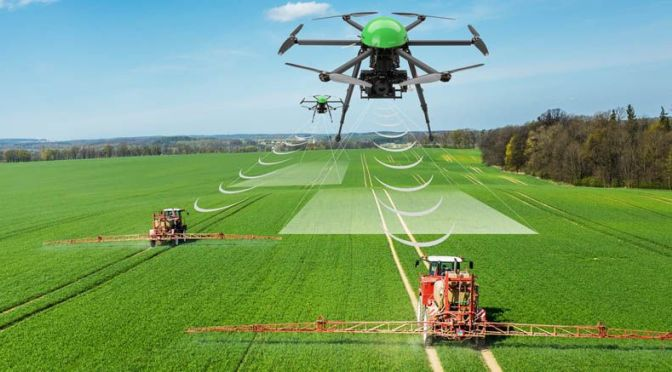
\includegraphics[scale=0.4]{drone-agricola.jpg}
\caption{Drone Agrícula \cite{drone}}
\label{fig:drone-agricola.jpg}
\end{figure}

\section{Relação com as outras disciplinas}
\quad A cadeira de Informática e Sociedade não possui pré-requisito e também não é pré-requisito de nenhuma outra disciplina.\cite{perfil} Porém, seu formato de ensino permite a discussão de temas relacionados a diversas matérias, permitindo aos seus alunos um breve conhecimento sobre as mesmas.

\bibliographystyle{unsrt}
\bibliography{thto}
\end{document}